\documentclass[landscape]{article}
\usepackage[a4paper,landscape,margin=1.5cm]{geometry}
\usepackage{graphicx}
\usepackage{array}
\usepackage{tabularx}
\usepackage{colortbl}
\usepackage{xcolor}
\usepackage{fancyhdr}
\usepackage{tikz}
\usepackage{booktabs}
\usepackage{subcaption}
\usepackage{pagecolor}
\usepackage{multirow}
\usepackage{lastpage}
\usepackage{tgheros} % Modern sans-serif font
\usepackage{setspace}
\usepackage[T1]{fontenc}
\usepackage{makecell}
\usepackage{enumitem} % Better list control
\usepackage{fontawesome5} % For icons
\usepackage{pdflscape} % Better landscape handling

\graphicspath{{illustration/}{reference/}{figures/}}  % Paths for images

% Define refined color palette
\definecolor{primaryblue}{RGB}{41, 65, 94}   % Deeper blue for main headers
\definecolor{secondaryblue}{RGB}{78, 112, 155} % Lighter blue for secondary elements
\definecolor{lightblue}{RGB}{235, 242, 250} % Very light blue for table backgrounds
\definecolor{mediumblue}{RGB}{120, 150, 180} % Medium blue for table headers
\definecolor{accentgold}{RGB}{216, 181, 109} % Gold accent color
\definecolor{backgroundbeige}{RGB}{252, 250, 245} % Light beige background
\definecolor{tablehead}{RGB}{245, 245, 245} % Subtle gray for table headers
\definecolor{bordercolor}{RGB}{220, 220, 220} % Subtle border color
\definecolor{subtleshadow}{RGB}{240, 240, 240} % For subtle shadows

% Set background color
\pagecolor{white}

% Set document font to sans-serif
\renewcommand{\familydefault}{\sfdefault}

% Better spacing
\setstretch{1.2}
\setlength{\parindent}{0pt}
\setlength{\parskip}{8pt}
\renewcommand{\arraystretch}{1.5} % Improve table row height globally

% Fix for table line alignment
\setlength{\arrayrulewidth}{0.5pt}
\setlength{\tabcolsep}{6pt}

% Custom page style
\pagestyle{fancy}
\fancyhf{}
\renewcommand{\headrulewidth}{0pt}
\renewcommand{\footrulewidth}{0pt}

% Enhanced Header with brand bar and subtle shadow
\fancyhead[C]{%
\begin{tikzpicture}[remember picture, overlay]
    % Shadow effect
    \fill[subtleshadow] 
        ([yshift=-1.2cm, xshift=0.2cm]current page.north west) rectangle 
        ([yshift=-0.8cm, xshift=0.2cm]current page.north east);
    
    % Header bar with gradient
    \shade[top color=primaryblue, bottom color=secondaryblue] 
        ([yshift=-1cm]current page.north west) rectangle 
        ([yshift=0cm]current page.north east);
    
    % Gold accent line
    \fill[accentgold] 
        ([yshift=-1cm]current page.north west) rectangle 
        ([yshift=-0.9cm]current page.north east);
    
    % Brand name with logo placeholder
    \node[anchor=west, text=white, font=\Large\bfseries] 
        at ([xshift=1cm, yshift=-0.5cm]current page.north west) 
        {J.Lindeberg};
    
    % Document type indicator
    \node[anchor=east, text=white, font=\large] 
        at ([xshift=-1cm, yshift=-0.5cm]current page.north east) 
        {TECHNICAL SPECIFICATION};
\end{tikzpicture}%
}

% Enhanced footer with contact info and modern design
\fancyfoot[C]{%
\begin{tikzpicture}[remember picture, overlay]
    % Shadow effect
    \fill[subtleshadow] 
        ([yshift=0.9cm, xshift=0.2cm]current page.south west) rectangle 
        ([yshift=0.2cm, xshift=0.2cm]current page.south east);
    
    % Blue footer bar with gradient
    \shade[bottom color=primaryblue, top color=secondaryblue] 
        ([yshift=0.7cm]current page.south west) rectangle 
        ([yshift=0cm]current page.south east);
    
    % Gold accent line
    \fill[accentgold] 
        ([yshift=0.7cm]current page.south west) rectangle 
        ([yshift=0.65cm]current page.south east);
    
    % Copyright text with icon
    \node[anchor=west, text=white, font=\small] 
        at ([xshift=1cm, yshift=0.35cm]current page.south west) 
        {\faIcon{copyright} J.Lindeberg 2025};
    
    % Contact info in footer
    \node[anchor=center, text=white, font=\small] 
        at ([yshift=0.35cm]current page.south) 
        {\quad};
    
    % Page number with icon
    \node[anchor=east, text=white, font=\small] 
        at ([xshift=-1cm, yshift=0.35cm]current page.south east) 
        {\faIcon{file-alt} PAGE \thepage\ OF \pageref{LastPage}};
\end{tikzpicture}%
}

% Improved section command with shadow effect
\newcommand{\techsection}[1]{%
\noindent\begin{tabularx}{\textwidth}{|X|}
\hline
\cellcolor{primaryblue}\textcolor{white}{\large\textbf{\faIcon{angle-right} #1}} \\
\hline
\end{tabularx}
\vspace{0.1cm}
}

% Command for elevated panels with shadow
\newcommand{\elevatedbox}[1]{%
\begin{tikzpicture}
\node[draw=bordercolor, line width=0.5pt, inner sep=10pt, fill=white, rounded corners=3pt, 
      drop shadow={shadow xshift=1pt, shadow yshift=-1pt, opacity=0.2}] {#1};
\end{tikzpicture}
}

\begin{document}

% Title with enhanced decorative elements and subtle shadow
\begin{center}

\begin{tikzpicture}
% Shadow layer
\node[inner sep=12pt, opacity=0.1, yshift=-2pt, xshift=2pt] (shadow) {\Huge\textbf{\textcolor{black}{Technical Specification Sheet}}};
% Main title
\node[inner sep=12pt] (title) {\Huge\textbf{\textcolor{primaryblue}{Technical Specification Sheet}}};
% Dual accent lines
\draw[accentgold, line width=2pt] ([yshift=-5pt]title.south west) -- ([yshift=-5pt]title.south east);
\draw[secondaryblue, line width=1pt] ([yshift=-9pt]title.south west) -- ([yshift=-9pt]title.south east);
% Icon decorations on both sides
\node[anchor=east, xshift=-10pt] at (title.west) {\textcolor{accentgold}{\Large\faIcon{ruler}}};
\node[anchor=west, xshift=10pt] at (title.east) {\textcolor{accentgold}{\Large\faIcon{cut}}};
\end{tikzpicture}
\end{center}

\vspace{0.5cm}

% PRODUCT DETAILS - Enhanced with icons and better layout
\begin{center}
\begin{tabular}{|>{\bfseries\raggedright\arraybackslash}p{3.2cm}|p{4cm}|>{\bfseries\raggedright\arraybackslash}p{3.2cm}|p{4cm}|}
\hline
\rowcolor{tablehead}\faIcon{tag} Brand: & J.Lindeberg & \rowcolor{tablehead}\faIcon{user} Designer: & APA \\
\hline
\faIcon{tshirt} Style Name: & Men's Leather Jacket & \faIcon{hashtag} Style Number: & JL-501 \\
\hline
\rowcolor{tablehead}\faIcon{layer-group} Category: & Jackets & \rowcolor{tablehead}\faIcon{calendar-alt} Season: & FW 2024 \\
\hline
\faIcon{calendar-day} Date: & October 7, 2023 & \faIcon{code-branch} Version: & 1.0 \\
\hline
\end{tabular}
\end{center}

\vspace{0.5cm}

% PRODUCT DESCRIPTION with elevated design
\begin{center}
\begin{tabular}{|p{14cm}|}
\hline
\rowcolor{tablehead}\multicolumn{1}{|c|}{\textbf{\faIcon{info-circle} PRODUCT DESCRIPTION}} \\
\hline
\vspace{0.2cm}
\large The jacket is crafted from premium leather, featuring a structured silhouette with a modern flair. A stand-up collar and front zip closure provide a sleek and functional design. The ribbed hem and cuffs not only offer comfort but also showcase a distinctive bomber aesthetic. The jacket’s interior is fully lined for added warmth and comfort. Ideal for both casual and semi-formal occasions, the design exudes versatility for everyday wear.
\vspace{0.3cm} \\
\hline
\end{tabular}
\end{center}

\newpage

% --------------------------------- FRONT VIEW SECTION ---------------------------------
\techsection{FRONT VIEW}
\vspace{-0.3cm}

\begin{tabular}{p{0.49\textwidth}|p{0.49\textwidth}}
% Left side - FRONT VIEW with better frame
\begin{center}
\begin{tikzpicture}
\node[draw=bordercolor, line width=0.5pt, inner sep=4pt, fill=white, rounded corners=3pt] {
    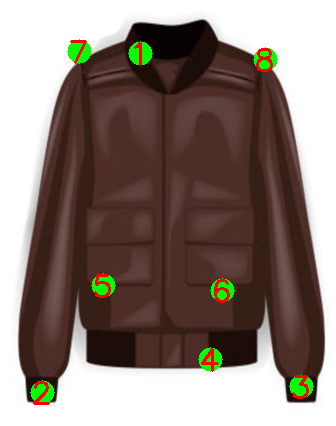
\includegraphics[width=0.35\textwidth,height=12cm,keepaspectratio]{jacket_front.png}
};
% Add a small label on top
\node[anchor=north, fill=accentgold, text=white, font=\small\bfseries, rounded corners=2pt, inner sep=2pt] 
    at ([yshift=0.5cm]current bounding box.north) {FRONT VIEW};
\end{tikzpicture}
\end{center}
&
% Right side - Attributes Table FRONT VIEW with improved formatting
\begin{center}
\begin{tabular}{|>{\columncolor{lightblue}\bfseries}p{3.5cm}|p{7cm}|}
\hline
\rowcolor{mediumblue}\multicolumn{1}{|c|}{\textcolor{white}{\textbf{\faIcon{list} Component}}} & \multicolumn{1}{c|}{\textcolor{white}{\textbf{\faIcon{info} Specifications}}} \\
\hline
1. Collar & A ribbed collar that stands about 2 cm tall, offering a snug fit. It is double-stitched at the base for extra durability. \\
\hline
2. Left Cuff & A ribbed cuff on the left sleeve with reinforced seams. The inside seam is finished with a serged edge for comfort. \\
\hline
3. Right Cuff & A matching ribbed cuff on the right sleeve. It is also reinforced and finished with a clean serged hem. \\
\hline
4. Waist Band & A stretchable ribbed waistband that snugly fits around the waist. Topstitching secures the band to the body for shape retention. \\
\hline
5. Left Pocket & A flap pocket with topstitched edges on the left side. Reinforced bartacks at stress points help prevent tearing. \\
\hline
6. Right Pocket & A flap pocket with topstitched edges on the right side. Bartacks at each corner provide additional strength under load. \\
\hline
7. Left Shoulder & A slightly sloped shoulder seam on the left. Twill tape reinforcement is used to maintain shape over time. \\
\hline
8. Right Shoulder & A matching right shoulder seam with similar reinforcement. The seam is carefully aligned for a balanced fit. \\
\hline
\end{tabular}
\end{center}
\end{tabular}

\vspace{0.5cm}

% MEASUREMENTS TABLE FRONT VIEW - WITH IMPROVED STYLING
\noindent\begin{tabularx}{\textwidth}{|>{\columncolor{lightblue}\bfseries}X|X|>{\centering\arraybackslash}X|>{\centering\arraybackslash}X|>{\centering\arraybackslash}X|>{\centering\arraybackslash}X|}
\hline
\rowcolor{primaryblue}\multicolumn{6}{|c|}{\textcolor{white}{\large\textbf{\faIcon{ruler-combined} FRONT MEASUREMENTS}}} \\
\hline
\rowcolor{mediumblue}\textcolor{white}{\textbf{Component}} & \textcolor{white}{\textbf{XS}} & \textcolor{white}{\textbf{S}} & \textcolor{white}{\textbf{M}} & \textcolor{white}{\textbf{L}} & \textcolor{white}{\textbf{XL}} \\
\hline
Shoulder Width (Keypoints #7-#8): Measured across shoulders at the front & 38\,cm & 40\,cm & 42\,cm & 44\,cm & 46\,cm \\
\hline
Chest Circumference (Keypoints #5-#6): Measured around the fullest part of the chest & 88\,cm & 92\,cm & 96\,cm & 100\,cm & 104\,cm \\
\hline
Waist Circumference (Keypoint #4): Measured at the top of the waistband & 80\,cm & 84\,cm & 88\,cm & 92\,cm & 96\,cm \\
\hline
Sleeve Length (Keypoints #2-#3): From shoulder seam to cuff edge & 60\,cm & 62\,cm & 64\,cm & 66\,cm & 68\,cm \\
\hline
Front Length (Keypoints #1-#4): From collar seam to bottom of waistband & 55\,cm & 57\,cm & 59\,cm & 61\,cm & 63\,cm \\
\hline
Pocket Depth (Keypoints #5-#6): From top edge of pocket flap to bottom edge & 15\,cm & 15\,cm & 16\,cm & 16\,cm & 17\,cm \\
\hline
\end{tabularx}
% ---------------------------------------------------------------------------------------------
\newpage

% --------------------------------- BACK VIEW SECTION ---------------------------------
\techsection{BACK VIEW}
\vspace{-0.3cm}

\begin{tabular}{p{0.49\textwidth}|p{0.49\textwidth}}
% Left side - BACK VIEW with better frame
\begin{center}
\begin{tikzpicture}
\node[draw=bordercolor, line width=0.5pt, inner sep=4pt, fill=white, rounded corners=3pt] {
    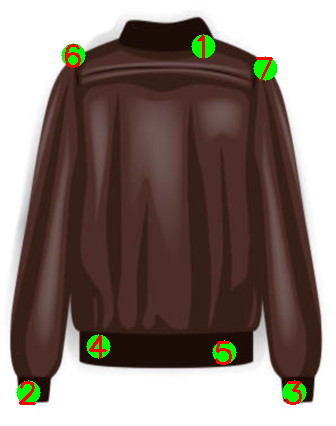
\includegraphics[width=0.35\textwidth,height=12cm,keepaspectratio]{jacket_back.png}
};
% Add a small label on top
\node[anchor=north, fill=accentgold, text=white, font=\small\bfseries, rounded corners=2pt, inner sep=2pt] 
    at ([yshift=0.5cm]current bounding box.north) {BACK VIEW};
\end{tikzpicture}
\end{center}
&
% Right side - Attributes Table BACK VIEW with improved formatting
\begin{center}
\begin{tabular}{|>{\columncolor{lightblue}\bfseries}p{3.5cm}|p{7cm}|}
\hline
\rowcolor{mediumblue}\multicolumn{1}{|c|}{\textcolor{white}{\textbf{\faIcon{list} Component}}} & \multicolumn{1}{c|}{\textcolor{white}{\textbf{\faIcon{info} Specifications}}} \\
\hline
1. Collar & A continuation of the ribbed collar at the back of the neckline. The seam at the back is carefully taped for smoothness. \\
\hline
2. Left Cuff & The same ribbed design as the front, with secure stitching. Ensures consistent look and fit from front to back. \\
\hline
3. Right Cuff & Matches the left cuff in design and construction. Reinforced to handle stretching over time. \\
\hline
4. Waist Band & The ribbed waistband wraps around the back. Secured with multiple rows of topstitching for durability. \\
\hline
5. Center Waist Tab & A small, reinforced tab at the center back waistband. Typically used for adjustable waist or brand labeling. \\
\hline
6. Left Shoulder Seam & Slightly dropped seam at the left shoulder for ease of movement. Stabilized with tape to prevent stretching. \\
\hline
7. Right Shoulder Seam & Mirror image of the left shoulder seam. Provides symmetrical shaping and balanced fit. \\
\hline
\end{tabular}
\end{center}
\end{tabular}

\vspace{0.5cm}

% MEASUREMENTS TABLE BACK VIEW - WITH IMPROVED STYLING
\noindent\begin{tabularx}{\textwidth}{|>{\columncolor{lightblue}\bfseries}X|X|>{\centering\arraybackslash}X|>{\centering\arraybackslash}X|>{\centering\arraybackslash}X|>{\centering\arraybackslash}X|}
\hline
\rowcolor{primaryblue}\multicolumn{6}{|c|}{\textcolor{white}{\large\textbf{\faIcon{ruler-combined} BACK MEASUREMENTS}}} \\
\hline
\rowcolor{mediumblue}\textcolor{white}{\textbf{Component}} & \textcolor{white}{\textbf{XS}} & \textcolor{white}{\textbf{S}} & \textcolor{white}{\textbf{M}} & \textcolor{white}{\textbf{L}} & \textcolor{white}{\textbf{XL}} \\
\hline
Back Shoulder Width (Keypoints #6-#7): Measured across the upper back & 38\,cm & 40\,cm & 42\,cm & 44\,cm & 46\,cm \\
\hline
Center Back Length (Keypoints #1-#4): From the collar seam down to the hem & 56\,cm & 58\,cm & 60\,cm & 62\,cm & 64\,cm \\
\hline
Sleeve Length (Keypoints #2-#3): Measured from the back shoulder seam to the cuff & 60\,cm & 62\,cm & 64\,cm & 66\,cm & 68\,cm \\
\hline
Across Back (Keypoint #5): Measured between the back armholes at mid-scapular level & 36\,cm & 38\,cm & 40\,cm & 42\,cm & 44\,cm \\
\hline
Armhole Depth (Keypoints #6-#7): From top of shoulder to underarm seam & 22\,cm & 23\,cm & 24\,cm & 25\,cm & 26\,cm \\
\hline
Neck Opening (Keypoint #1): Circumference of the ribbed collar at back & 40\,cm & 41\,cm & 42\,cm & 43\,cm & 44\,cm \\
\hline
\end{tabularx}
% ---------------------------------------------------------------------------------------------
\newpage

% REFERENCE IMAGES SECTION with callouts
\techsection{REFERENCE}
\vspace{-0.3cm}

\begin{tabular}{p{0.49\textwidth}|p{0.49\textwidth}}
% Left side - Place reference images with annotations
\begin{center}
\begin{tikzpicture}
\node[draw=bordercolor, line width=0.5pt, inner sep=4pt, fill=white, rounded corners=3pt] (img) {
    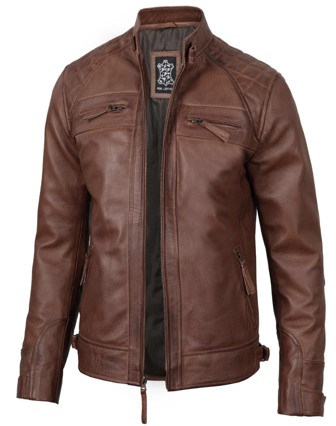
\includegraphics[width=0.35\textwidth,height=12cm,keepaspectratio]{jacket_reference.png}
};

% Sample callout annotations (uncomment and modify when image is added)
%\draw[accentgold, ->, line width=1pt] (1,1) -- (0.5,0.5) node[right, text=black, font=\small, align=left, xshift=5pt] {Special detail};
%\draw[accentgold, ->, line width=1pt] (-1,1) -- (-0.5,0.5) node[left, text=black, font=\small, align=right, xshift=-5pt] {Stitch detail};

% Add a small label on top
\node[anchor=north, fill=accentgold, text=white, font=\small\bfseries, rounded corners=2pt, inner sep=2pt] 
    at ([yshift=0.5cm]current bounding box.north) {INSPIRATION \& DETAILS};
\end{tikzpicture}
\end{center}
&
% Right side - Description of reference image with enhanced formatting
\begin{center}
\begin{tabular}{|p{10cm}|}
\hline
\rowcolor{mediumblue}\multicolumn{1}{|c|}{\textcolor{white}{\textbf{\faIcon{lightbulb} Design Inspiration \& Notes}}} \\
\hline
\begin{minipage}[t]{\linewidth}
\vspace{0.3cm}
A sleek, structured leather jacket that balances both style and functionality.
\begin{itemize}[leftmargin=*, label={\textcolor{accentgold}{\faIcon{check-circle}}}]
  \item Premium brown leather with subtle texture
  \item Additional zippered pockets for secure storage
  \item Minimal collar design reminiscent of a stand-collar style
\end{itemize}
\vspace{0.3cm}
\end{minipage} \\
\hline
\end{tabular}
\end{center}
\end{tabular}

\newpage

% BILL OF MATERIALS with enhanced design
\techsection{BILL OF MATERIALS}
\vspace{-0.3cm}
\noindent\begin{tabularx}{\textwidth}{|>{\columncolor{lightblue}\bfseries}p{3cm}|X|>{\raggedleft\arraybackslash}p{2.5cm}|>{\raggedleft\arraybackslash}p{2.5cm}|}
\hline
\rowcolor{mediumblue}\textcolor{white}{\textbf{Material}} & \textcolor{white}{\textbf{Description}} & \textcolor{white}{\textbf{Unit Cost}} & \textcolor{white}{\textbf{Total Cost}} \\
\hline
Leather (1.2mm thick) & Full-grain hide & 50.00 & 100.00 \\
\hline
Polyester Lining & Smooth finish & 3.00 & 6.00 \\
\hline
Rib Knit (Hem \& Cuffs) & Cotton-Spandex blend & 2.50 & 5.00 \\
\hline
Metal Zippers & YKK brand \#5 & 2.00 & 4.00 \\
\hline
Snap Buttons & Reinforced metal & 1.00 & 1.00 \\
\hline
Sewing Thread & High-tensile polyester & 0.50 & 1.00 \\
\hline
Interfacing & Lightweight fusible & 1.50 & 1.50 \\
\hline
Woven Label & Brand label & 0.50 & 0.50 \\
\hline
\multicolumn{3}{|r|}{\textbf{Total Material Cost:}} & 119.00 \\
\hline
\end{tabularx}

\vspace{0.7cm}

\newpage

% CARE INSTRUCTIONS with icons
\techsection{CARE INSTRUCTIONS}
\vspace{-0.3cm}

\noindent\begin{tabularx}{\textwidth}{|X|}
\hline
\begin{minipage}[t]{\linewidth}
\vspace{0.3cm}
\large 
\begin{center}
\begin{tabular}{ccccc}
\textcolor{primaryblue}{\Large\faIcon{ban}} & 
\textcolor{primaryblue}{\Large\faIcon{ban}} & 
\textcolor{primaryblue}{\Large\faIcon{ban}} & 
\textcolor{primaryblue}{\Large\faIcon{ban}} & 
\textcolor{primaryblue}{\Large\faIcon{store}} \\
No Machine Wash & No Bleach & No Tumble Dry & No Iron & Specialist Leather Clean \\
\end{tabular}
\end{center}
\vspace{0.3cm}
\end{minipage} \\
\hline
\end{tabularx}

\vspace{0.7cm}

% ADDITIONAL COMMENTS with improved formatting
\techsection{ADDITIONAL COMMENTS}
\vspace{-0.3cm}
\noindent\begin{tabularx}{\textwidth}{|X|}
\hline
\begin{minipage}[t]{\linewidth}
\vspace{0.3cm}
\large 
% (Left blank intentionally)
\vspace{0.3cm}
\end{minipage} \\
\hline
\end{tabularx}

\vspace{0.7cm}
% SIGNATURES
\techsection{SIGNATURES}
\vspace{-0.3cm}
\noindent\begin{tabularx}{\textwidth}{|X|}
\hline
\begin{minipage}[t]{\linewidth}
\vspace{0.3cm}
\large\textbf{Approvals:} \underline{\hspace{5cm}} (Design Director) \hspace{1cm} \underline{\hspace{5cm}} (Production Manager)
\vspace{0.3cm}
\end{minipage} \\
\hline
\end{tabularx}

\newpage

% DISCLAIMER AND CONFIDENTIALITY
\begin{center}
\begin{tabular}{|p{23cm}|}
\hline
\rowcolor{primaryblue}\multicolumn{1}{|c|}{\textcolor{white}{\textbf{DISCLAIMER AND CONFIDENTIALITY}}} \\
\hline
\large This Technical Specification Sheet, including all designs, measurements, and related information, is the confidential and proprietary property of J.Lindeberg. Any unauthorized disclosure, copying, distribution, or use of the contents herein is strictly prohibited. J.Lindeberg reserves the right to modify the design, materials, and construction without prior notice. By reviewing this document, you agree to maintain its confidentiality and refrain from sharing it with any third party without explicit written consent from J.Lindeberg.
\\
\hline
\end{tabular}
\end{center}

\end{document}
